\documentclass[11pt]{scrartcl}
\usepackage{fullpage}

\usepackage{cite}
%\usepackage{pbox}
\usepackage{soul}
%\usepackage{showkeys}

\usepackage{listings} % Coding Syntax coloring
\usepackage{color}
\usepackage{textcomp}
\definecolor{listinggray}{gray}{0.9}
\definecolor{lbcolor}{rgb}{0.9,0.9,0.9}
\usepackage{amsmath}
\usepackage{textcomp}

\lstset{
     backgroundcolor=\color{lbcolor},
     tabsize=4,
     rulecolor=,
     language=matlab,
        basicstyle=\scriptsize,
        upquote=true,
        aboveskip={1.5\baselineskip},
        columns=fixed,
        showstringspaces=false,
        extendedchars=true,
        breaklines=true,
        prebreak = \raisebox{0ex}[0ex][0ex]{\ensuremath{\hookleftarrow}},
        frame=single,
        showtabs=false,
        showspaces=false,
        showstringspaces=false,
        identifierstyle=\ttfamily,
        keywordstyle=\color[rgb]{0,0,1},
        commentstyle=\color[rgb]{0.133,0.545,0.133},
        stringstyle=\color[rgb]{0.627,0.126,0.941},
}
\usepackage{fancyhdr,graphicx,lastpage}% http://ctan.org/pkg/{fancyhdr,graphicx,lastpage}
\fancypagestyle{plain}{
  \fancyhf{}% Clear header/footer
  \fancyhead[R]{
\includegraphics[scale=0.5]{logo.png}}% Right header
  \fancyhead[L]{\textbf{School of Electronic and Electrical Engineering}}
  %\fancyfoot[L]{Name Firstname - v1.0 \\  Date}% Left footer
  \fancyfoot[R]{\thepage\  / \pageref{LastPage}}% Right footer
}
\pagestyle{plain}% Set page style to plain.


\begin{document}

\title{ELEC 2520 Energy Systems and control}
\subtitle{ LAB REPORT 3: MATLAB Simulation of Linear Systems}
\author{Yingjie Luan(200829024)}
\maketitle

%\begin{tabular}{cc}
%    \begin{minipage}{.5\linewidth}
%        \begin{tabular}{|c|c|}
%        \hline
%        Student Name & Student ID \\
%        \hline
%        Yingjie Luan & 200829024 \\
%        \hline
%        \end{tabular}
%    \end{minipage} &
%
%    \begin{minipage}{.5\linewidth}
%        \begin{tabular}{|c|c|c|c|}
%        \hline
%        \pbox{20cm}{Mark for \\ Content} & \pbox{20cm}{Mark for \\ Presentation} &\pbox{20cm}{Mark for \\ Conciseness} & \textbf{Total} \\
%        \hline
%        \multicolumn{1}{|r}{/50} & \multicolumn{1}{|r|}{/10} &\multicolumn{1}{|r|}{/10}&\multicolumn{1}{r|}{/70} \\
%        \hline
%        \end{tabular}
%    \end{minipage} 
%\end{tabular}

\textbf{Full marks will only be given if your calculations, derivation of formula and results have been explained clearly. If additional space is needed, please attach separate sheet(s). Note that a high quality report which deserves a good mark is the one that has legible writing, well-sorted equations and well-presented diagrams. This report can be typed out and diagrams can be computer generated if that helps you to produce a more presentable report. You may complete this report in your own time and submit it through VLE by \underline{11:59 pm Friday (24thApril 2015).} }
%\tableofcontents

\section*{Section 3 Constant Gain Position-Feedback Control}


\subsection*{a}
\textbf{ Sketch a few of the graphs obtained, and comment on how you selected k3 so that the design requirements can be satisfied (OR as much as possible). Our requirements here are that Vo(t) should settle to its steady-state value within one second and should not overshoot by more than 10\% (with respect to its steady-state value).}\\


Below is a colormap version of the plot, in total, 50 lines were drawn:\\
\begin{minipage}[t]{\linewidth}

{
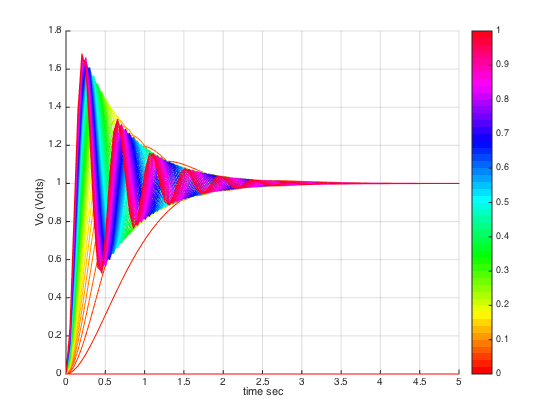
\includegraphics[scale = 0.7]{main.png}
\captionof{figure}{This is the colormap of the plot.}
\label{fig:main}
}
\end{minipage}
\medskip

As we can see, the steady state value should be 1, so to testify the second requirement(which is to find the overshoot no more than 10\%) is easy. After applying a filter at the front, we then can find that:

\begin{minipage}[t]{\linewidth}

{
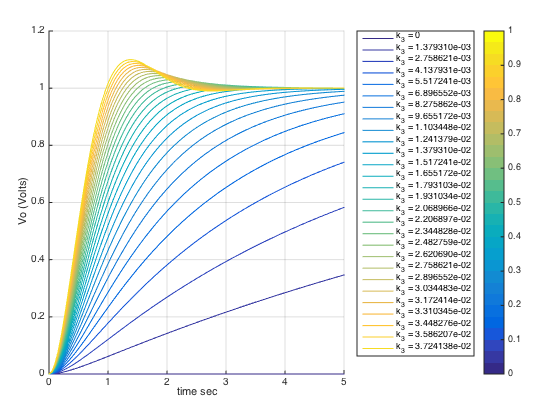
\includegraphics[scale = 0.7]{main_4.png}
\captionof{figure}{This is value of $k_3$ making sure overshoot no more than 10\%.}
\label{fig:main_2}
}
\end{minipage}
\medskip

As we can see from figure\ref{fig:main_2}, that the value of ${k_3}$ should range from 0.01 to 0.04. So I decide to plot some figures within that range.

Below is a plot within that range:\\
\begin{minipage}[t]{\linewidth}

{
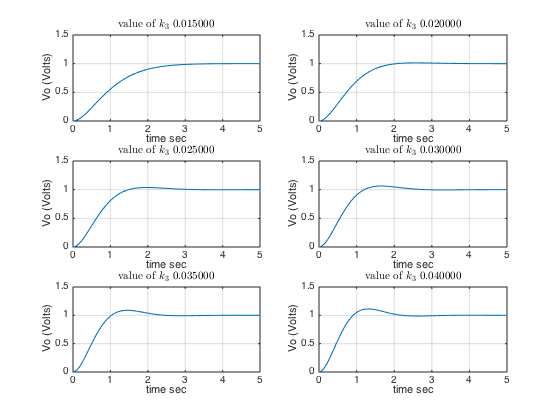
\includegraphics[scale = 0.7]{main_5.png}
\captionof{figure}{There are the plots of a range of $k_3$. As we can see,}
%\label{fig:main_2}
}
\end{minipage}
\medskip

So after the above experiment, the conclusion is that I felt it is hard to fulfill the above requirement. The closest value of $k_3$ can be 0.03, which settle to its steady-state just a bit later than one second. Further, as we can see from figure\ref{fig:main_2}, that none of the value of $k_3$ actually settle to its steady state value early than one second.
\subsection *{b}
\textbf{Using the information in Figure 1 of your lab sheet, with no tacho-feedback (ONLY CONSIDERING THE OUTER LOOP), derive the closed-loop transfer function for Constant Gain Position-Feedback Control. You should present AND explain your derivation systematically. }

\begin{center}
$$ \text{Close loop gain} = \frac{\text{forward path gain}}{1+\text{open loop gain}} $$
\end{center}

The forward path gain and the open loop gain is the same, which is :
\begin{center}
$$ k_ek_3k_a\frac{k_m}{1+sT_m}k_g\frac{k_p}{s}$$
\end{center}

Put in the formula:

It is :

\begin{eqnarray*}
 &=& \frac{k_ek_3k_a\frac{k_m}{1+sT_m}k_g\frac{k_p}{s}}{1+k_ek_3k_a\frac{k_m}{1+sT_m}k_g\frac{k_p}{s}}\\
 &=& \frac{\frac{k_3k_v}{1+sT_ms}}{1+\frac{k_3k_v}{1+sT_ms}}\\
 &=& \frac{k_3k_v}{s^2T_m+s+k_3k_v}\\
 &=& \frac{\frac{k_3k_v}{T_m}}{s^2+\frac{s}{T_m}+\frac{k_3k_v}{T_m}}
\end{eqnarray*}
Where $k_v = k_ek_ak_mk_gk_p $


\subsection*{c}
\label{ssec:cpart}

\textbf{Show that the design specifications (overshoot less than 10\% and settling time less than 1 second) cannot be achieved by only the Position Feedback. (Based on the normalised second order unit step responses, you may need to show some mathematical derivation and include your explanation below.)}\\

I first normalize the formula in the following format:
$$ \frac{1}{s^2\frac{T_m}{k_3k_v}+s\frac{1}{k_3k_v}+1}$$

According to the standard second-order system formula I find out the following is true:
$$\frac{1}{\omega_n^2}=\frac{T_m}{k_3k_v} $$ 
$$\frac{2\zeta}{\omega_n}=\frac{1}{k_3k_v}$$
We then can conduct that:

\begin{equation} \label{equ:omega}
\omega_n= \sqrt{\frac{k_3k_v}{T_m}}
\end{equation}

\begin{equation} \label{equ:zeta}
\zeta = \frac{1}{2\sqrt{T_mk_3k_v}}
\end{equation}

\begin{minipage}[t]{\linewidth}
\label{fig:main}

{
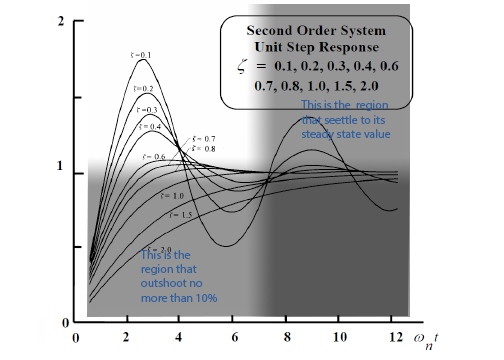
\includegraphics[scale = 1]{vis.png}
\captionof{figure}{This is figure to derive the standard for the system.}
}
\end{minipage}
\medskip

According to the above figure, we can get to the conclusion that $\zeta$ should be larger than 0.6.\\

And after applying this to formula \ref{equ:zeta}, I find out that we need $k_3 <=0.0362$.

At the meantime, if $k_3 <=0.0362$, $\omega_n$ will be less than 2.7790. But at the mean time from the provided figure we can see that we require $t*\omega$ larger than 5.5. And putting $t<=1$ we find out that we cannot find the qualified $\omega$. Summing up, there is no qualified $k_3$ value on this condition. Thus, just position control is not enough for this task. 

\section*{Section 4: Position and Velocity Feedback Control }

\subsection*{a}
\textbf{Using the information in Figure 1, with tacho-feedback (CONSIDERING BOTH INNER AND OUTER FEEDBACKS), derive the closed-loop transfer function for Constant Gain Position + Velocity Feedback Control. You should present AND explain your derivation systematically.}\\

According to the formula:
\begin{center}
$$ \text{Close loop gain} = \frac{\text{forward path gain}}{1+\text{open loop gain}} $$
\end{center}

The inner loop:\\

The forward path gain is:
$$k_ek_3k_ak_m\frac{k_m}{1+sT_m}$$

The closed loop gain is:
$$k_ek_3k_ak_m\frac{k_m}{1+sT_m}k_1k_T$$

Thus, the inner loop gain is :
$$\frac{k_ek_3k_ak_m}{1+s*T_m+k_ek_3k_ak_mk_1k_T}$$

Using the gain of the inner loop as a module, we can calculate the transfer function for the outer loop in the similar manner:

The forward path gain and the closed loop gain is :
$$\frac{k_ek_3k_ak_mk_g\frac{k_p}{s}}{1+s*T_m+k_ek_3k_ak_mk_1k_T}$$
The conduction of the outer loop gain:
\begin{eqnarray*}
&=&\frac{k_3k_v}{s((1+sT_m)+(k_ek_3k_ak_mk_1k_T))+k_3k_v}\\
&=&\frac{k_3k_v}{s^2T_m+s(1+\frac{k_vk_1k_Tk_3}{k_gk_p})+k_vk_3}\\
&=&\frac{\frac{k_3k_v}{T_m}}{s^2+s(\frac{1}{T_m}+\frac{k_vk_1k_Tk_3}{k_gk_pT_m})+\frac{k_vk_3}{T_m}}
\end{eqnarray*}
Where $k_v = k_ek_ak_mk_gk_p $

\subsection*{b}
\textbf{Explain how you selected $\omega_n$ and $\zeta$ from the normalised step responses to achieve the design specification of a step response that settles around 1 second with an overshoot less than 10\%.}\\

This has been mentioned in the section above. That we can see from the image below:

\begin{minipage}[t]{\linewidth}
\label{fig:main}

{
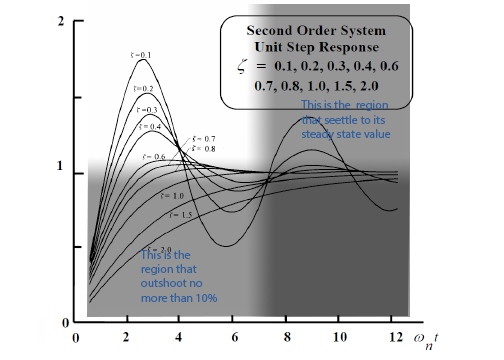
\includegraphics[scale = 1]{vis.png}
\captionof{figure}{This is figure to derive the standard for the system.}
}
\end{minipage}
\medskip

That only the overlapping part of the image satisfy the requirement. And to do so we need $\zeta >= 0.6$ and $\omega_n $ at least larger than 5.5(on condition that t is smaller than 1). 

\subsection*{c}
\textbf{What are the values of $k_3$ and $k_1$ which enable you to satisfy the design requirement? Using the closed-loop transfer function you have derived in Part (a) to confirm your results.}\\

Using the provided program \textit{sim2.m} and by calculating the value of $\omega_n$ and $\zeta$ back to $k_1$ and $k_3$, we get the following answers when $\zeta=0.6$ and $\omega_n=5.5$.
\begin{eqnarray*}
k_1&\approx&0.36\\
k_3&\approx& 0.1418
\end{eqnarray*}
Which are both in the range of [0,1] and thus we can adopt both of those values.

According to the normalized formula along with the standard second-order system response formula, we can get:
$$ \omega_n = \sqrt{\frac{k_3k_v}{T_m}}$$
$$\zeta = \frac{\frac{1}{T_m}+\frac{k_1k_3k_tk_v}{T_mk_pk_g}}{2\omega_n}$$

Putting in the value of $k_1$ and $k_3$ we can further get the value of $\omega_n$ and $\zeta$ which is:
\begin{eqnarray*}
\omega_n &\approx& 5.5001\\
\zeta &\approx& 0.6000
\end{eqnarray*}

Thus we further confirmed that the result should be qualified and in accordance with the standard graph.

Below is the response graph when the $k_1$ and $k_3$ adopts those two values:

\begin{minipage}[t]{\linewidth}

{
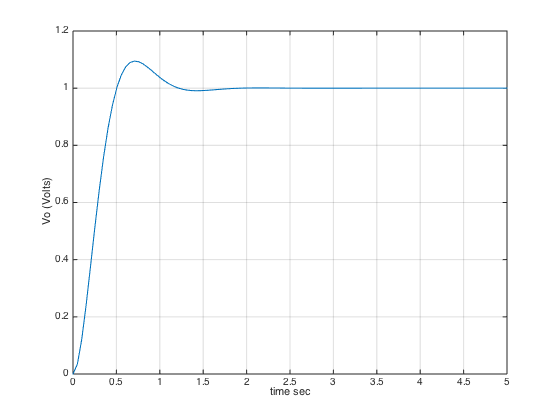
\includegraphics[scale = 0.7]{fig_4.png}
\captionof{figure}{This is the system response when $k_1=0.36$ and $k_3=0.1418$. As we can see, this system response roughly satisfied our two basic requirements.}
}
\end{minipage}
\medskip

Further, if we keeping increasing the standard of $\omega_n$ and $\zeta$ we can get a even better result, below is the result when we select $\omega_n=8$ and $\zeta=0.8$:\\

\begin{minipage}[t]{\linewidth}

{
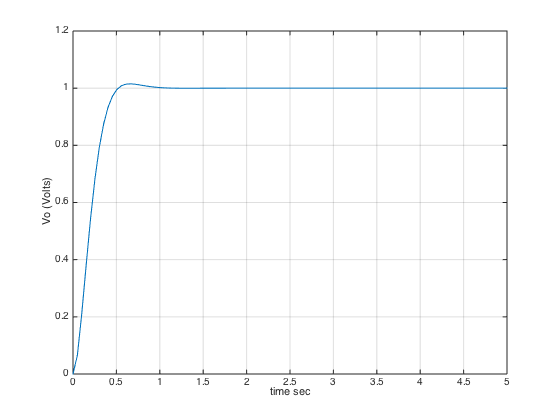
\includegraphics[scale = 0.7]{fig_5.png}
\captionof{figure}{This is the system response when $k_1\approx0.4931$ and $k_3\approx0.3$. As we can see, this system response have satisfied our two basic requirement.}
}
\end{minipage}
\medskip

The related $k_1\approx0.4931$ and $k_3\approx0.3$

\subsection*{d}
\textbf{Explain why velocity feedback helps to increase the damping of the system in this case.}\\

In simple, the velocity control give us a more dimension in controlling the system's response, when the $k_1$ equals to 0, we then can get the standard position control.\\

From the PID point of view, velocity is the differential of the system, and this derivative term can help predict system behavior and improve the system settling time and stability.\cite{ref_1} It acts to stabilize the transient response of the system, can be thought as electronic damping. However, the steady-state error is not affected.\cite{ref_2}


\bibliographystyle{plain}
\bibliography{bibliography} 

\end{document}
